% Paquets généraux
\documentclass[a4paper,12pt,titlepage]{article}
\usepackage[T1]{fontenc}
\usepackage[utf8]{inputenc}
\usepackage[french]{babel}
\usepackage[gen]{eurosym}
%\usepackage[dvips]{graphicx}
\usepackage{fancyhdr}
\usepackage{pdfpages} 
\usepackage{multido}
\usepackage{hyperref}
%\usepackage{textcomp}
%\usepackage{aeguill}
\usepackage{schemabloc}
\usepackage[bitstream-charter]{mathdesign}

\newcommand{\id}{54}
\newcommand{\nom}{Liaisons mécaniques}
\newcommand{\sequence}{04}
\newcommand{\num}{01}
\newcommand{\type}{TP}
\newcommand{\descrip}{Modélisation d'un solide. Comportement des liaisons mécaniques. Modéliser les mécanismes du laboratoire par un schéma cinématique, paramétré.}
\newcommand{\competences}{A3-C4: Analyse d'architecture et de comportement \\ &  Mod1-C1: Isolement d'un solide ou d'un système de solides \\ &  Mod2-C10-1: Modèle de solide indéformable \\ &  Mod2-C11: Modélisation géométrique et cinématique des mouvements entre solides indéformables \\ &  Mod2-C12: Modélisation cinématique des liaisons entre solides \\ &  Mod2-C15: Modélisation des actions mécaniques \\ &  Rés-C6: Utilisation d'un solveur ou d'un logiciel multi physique \\ &  Com1-C1: Différents descripteurs introduits dans le programme \\ &  Com2-C4: Outils de communication}
\newcommand{\nbcomp}{9}
\newcommand{\systemes}{Plateforme Stewart}
\newcommand{\systemessansaccent}{Plateforme Stewart}
\newcommand{\ilot}{2}
\newcommand{\ilotstr}{02}
\newcommand{\dossierilot}{\detokenize{Ilot_02 Plateforme Stewart}}
\newcommand{\imageun}{Plateforme}

\newcommand{\urlsysteme}{\href{https://www.costadoat.fr/systeme/57}{Ressources système}}
\newcommand{\matlabsimscape}{\href{https://github.com/Costadoat/Sciences-Ingenieur/raw/master/Systemes/Plateforme Stewart/Plateforme_Stewart_Simscape.zip}{Modèle Simscape}}
\newcommand{\solidworks}{\href{https://github.com/Costadoat/Sciences-Ingenieur/raw/master/Systemes/Plateforme Stewart/Plateforme_Stewart_Solidworks.zip}{Modèle Solidworks}}
\newcommand{\edrawings}{\href{https://github.com/Costadoat/Sciences-Ingenieur/raw/master/Systemes/Plateforme Stewart/Plateforme_Stewart.EASM}{Modèle eDrawings}}
\newcommand{\test}{Stewart_param1}
\newcommand{\testi}{Stewart_param2}
\newcommand{\testii}{Stewart_param3}
\newcommand{\testiii}{Stewart_param4}
\newcommand{\testiiii}{Stewart_euler}

\newcommand{\auteurun}{Renaud Costadoat}
\newcommand{\auteurdeux}{Françoise Puig}
\newcommand{\institute}{Lycée Dorian}


\usepackage{color}
\usepackage{xcolor}
\usepackage{colortbl}
\usepackage{helvet}
\renewcommand{\familydefault}{\sfdefault}
\usepackage{amsfonts}
\usepackage{amsmath}
%\usepackage{xspace}
\usepackage{varioref}
\usepackage{tabularx}
%\usepackage{floatflt}
\usepackage{graphics}
\usepackage{wrapfig}
\usepackage{textcomp}
\usepackage{tikz}
\usepackage{wrapfig}
\usepackage{gensymb}
\usepackage[european]{circuitikz}
\usetikzlibrary{babel}
\usepackage{ifthen}
\usepackage{cancel}
\usepackage{etoolbox}
\usepackage{multirow}
%\usepackage{boxedminipage}
\definecolor{gris25}{gray}{0.75}
\definecolor{bleu}{RGB}{18,33,98}
\definecolor{bleuf}{RGB}{42,94,171}
\definecolor{bleuc}{RGB}{231,239,247}
\definecolor{rougef}{RGB}{185,18,27}
\definecolor{rougec}{RGB}{255,188,204}%255,230,231
\definecolor{vertf}{RGB}{103,126,82}
\definecolor{vertc}{RGB}{220,255,191}
\definecolor{forestgreen}{rgb}{0.13,0.54,0.13}
\definecolor{blcr}{rgb}{0.59,0.69,0.84}
\definecolor{blfr}{rgb}{0.32,0.51,0.75}
\definecolor{orfr}{rgb}{0.90,0.42,0.15}
\definecolor{orcr}{rgb}{0.90,0.65,0.50}
\definecolor{orangef}{rgb}{0.659,0.269,0.072}
\definecolor{orange}{rgb}{0.58,0.35,0.063}
\definecolor{orangec}{rgb}{0.43,0.32,0.25}
\definecolor{rcorrect}{rgb}{0.6,0,0}
\definecolor{sequence}{rgb}{0.75,0.75,0.75}
\definecolor{competences}{rgb}{0.61,0.73,0.35}
\definecolor{grisf}{HTML}{222222}
\definecolor{grisc}{HTML}{636363}
\definecolor{normal}{HTML}{4087c4}
\definecolor{info}{HTML}{5bc0de}
\definecolor{success}{RGB}{92,184,92}
\definecolor{warning}{RGB}{240,173,78}
\definecolor{danger}{RGB}{217,83,79}
\hypersetup{                    % parametrage des hyperliens
    colorlinks=true,                % colorise les liens
    breaklinks=true,                % permet les retours à la ligne pour les liens trop longs
    urlcolor= blfr,                 % couleur des hyperliens
    linkcolor= orange,                % couleur des liens internes aux documents (index, figures, tableaux, equations,...)
    citecolor= forestgreen                % couleur des liens vers les references bibliographiques
    }

% Mise en page
\pagestyle{fancy}

\setlength{\hoffset}{-18pt}

\setlength{\oddsidemargin}{0pt} 	% Marge gauche sur pages impaires
\setlength{\evensidemargin}{0pt} 	% Marge gauche sur pages paires
\setlength{\marginparwidth}{00pt} 	% Largeur de note dans la marge
\setlength{\headwidth}{481pt} 	 	% Largeur de la zone de tête (17cm)
\setlength{\textwidth}{481pt} 	 	% Largeur de la zone de texte (17cm)
\setlength{\voffset}{-18pt} 		% Bon pour DOS
\setlength{\marginparsep}{7pt}	 	% Séparation de la marge
\setlength{\topmargin}{-30pt} 		% Pas de marge en haut
\setlength{\headheight}{35pt} 		% Haut de page
\setlength{\headsep}{20pt} 		% Entre le haut de page et le texte
\setlength{\footskip}{30pt} 		% Bas de page + séparation
\setlength{\textheight}{700pt} 		% Hauteur de l'icone zone de texte (25cm)
\setlength\fboxrule{1 pt}
\renewcommand{\baselinestretch}{1}
\setcounter{tocdepth}{1}
\newcommand{\cadre}[2]
{\fbox{
  \begin{minipage}{#1\linewidth}
   \begin{center}
    #2\\
   \end{center}
  \end{minipage}
 }
}

\newcounter{num_quest} \setcounter{num_quest}{0}
\newcounter{num_rep} \setcounter{num_rep}{0}
\newcounter{num_cor} \setcounter{num_cor}{0}

\newcommand{\question}[1]{\refstepcounter{num_quest}\par
~\ \\ \parbox[t][][t]{0.15\linewidth}{\textbf{Question \arabic{num_quest}}}\parbox[t][][t]{0.93\linewidth}{#1}\par
}


\newcommand{\reponse}[1]
{\refstepcounter{num_rep}
\noindent
\rule{\linewidth}{.5pt}
\textbf{Question \arabic{num_rep}:}
\multido{\i=1+1}{#1}{~\ \\}
}

\newcommand{\cor}
{\refstepcounter{num_cor}
\noindent
\rule{\linewidth}{.5pt}
\textbf{Question \arabic{num_cor}:} \\
}

\newcommand{\titre}[1]
{\begin{center}
\cadre{0.8}{\huge #1} 
\end{center}
}


% En tête et pied de page
\fancypagestyle{normal}{%
  \fancyhf{}
\lhead{\nom}
\rhead{
\includegraphics[width=2cm]{../../img/logo}\hspace{2pt}}
\ifdef{\auteurdeux}{\lfoot{\auteurun,\auteurdeux}}{\lfoot{\auteurun}}
\cfoot{Page \thepage}}

\fancypagestyle{correction}{%
  \fancyhf{}
  \lhead{\colorbox{danger}{\begin{minipage}{0.65\paperwidth} \textcolor{white}{\textbf{Correction}} \end{minipage}} }
  \rhead{
\includegraphics[width=2cm]{../../img/logo}}
  \ifdef{\auteurdeux}{\lfoot{\auteurun,\auteurdeux}}{\lfoot{\auteurun}}
  \rfoot{\colorbox{danger}{\begin{minipage}{0.5\paperwidth} \begin{flushright}\textcolor{white}{\textbf{Correction}}\end{flushright} \end{minipage}} }}

\renewcommand{\footrulewidth}{0.4pt}

\usepackage{eso-pic}
\newcommand{\BackgroundPic}{%
\put(0,0){%
\parbox[b][\paperheight]{\paperwidth}{%
\vfill
\begin{center}
\hspace{0.5cm}\vspace{0.5cm}

\includegraphics[width=\paperwidth,height=\paperheight,%
keepaspectratio]{../../img/fond3}%
\end{center}
\vfill
}}}

\newcommand{\BackgroundPicdeux}{%
\put(25,-30){%
\parbox[b][\paperheight]{\paperwidth}{%
\vfill
\begin{center}
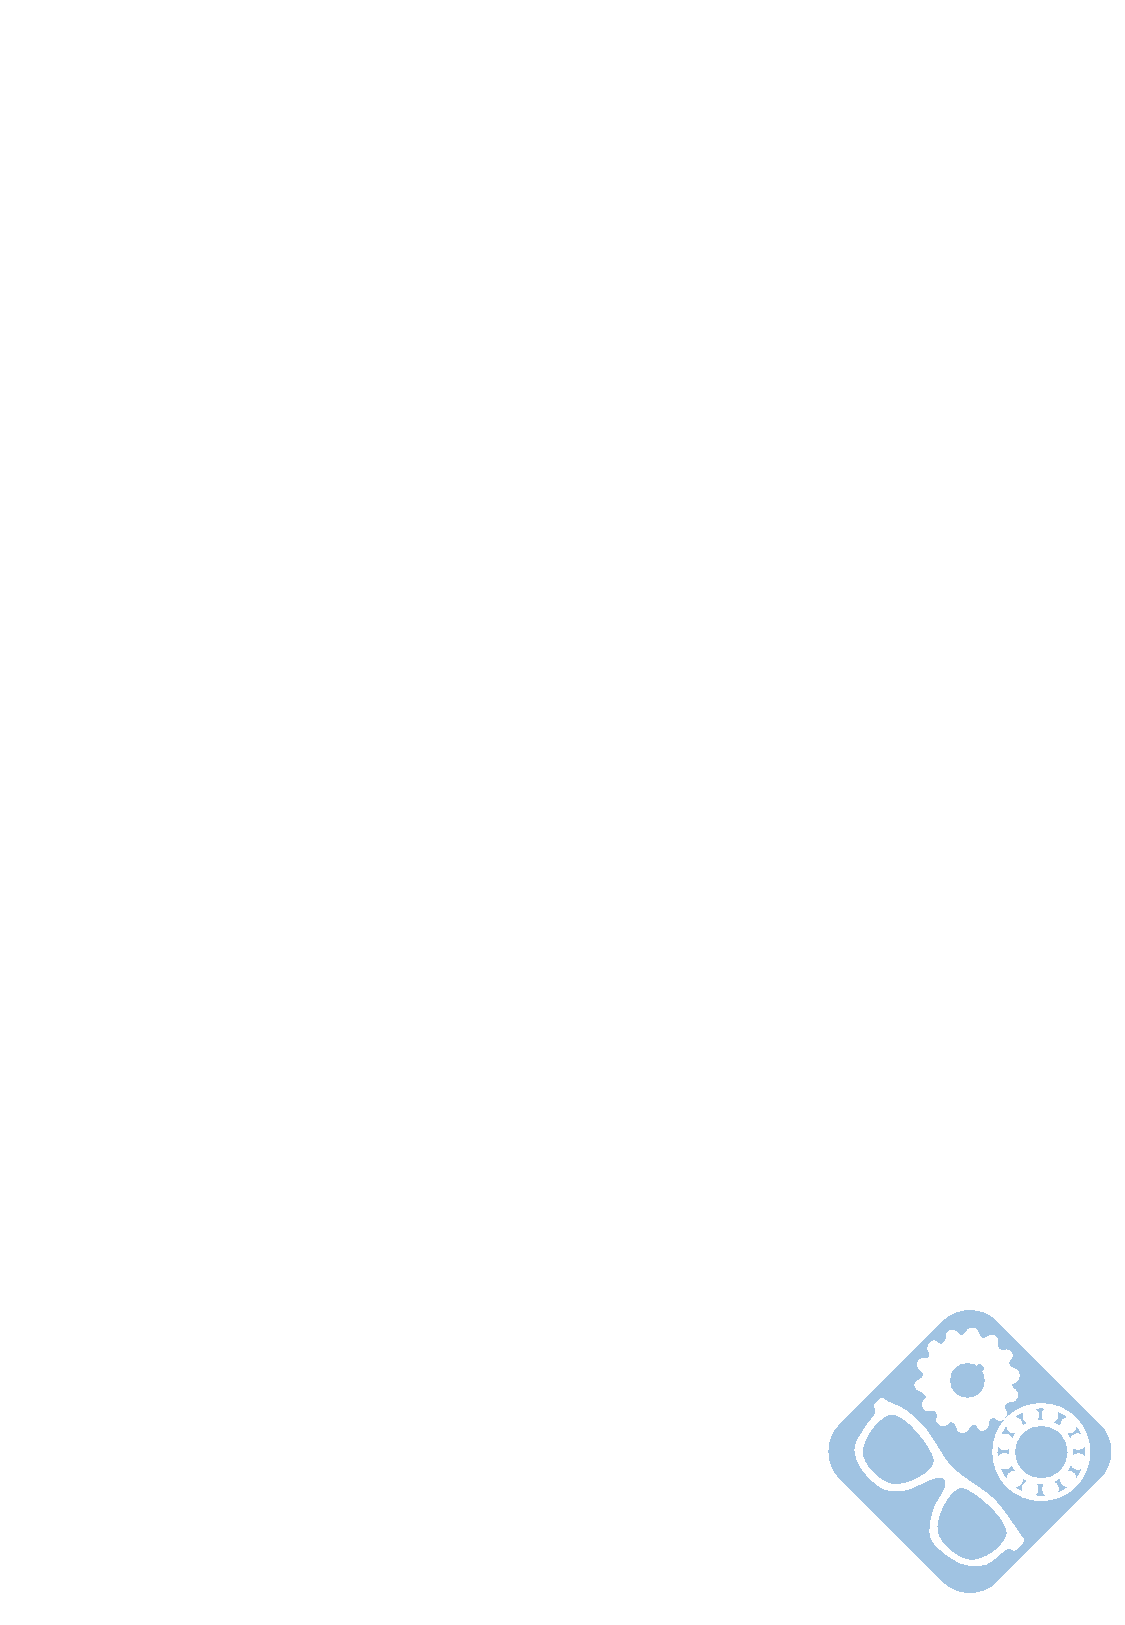
\includegraphics[width=\paperwidth,height=\paperheight,%
keepaspectratio]{../../img/fond4}%
\end{center}
\vfill
}}}

\begin{document}

\pagestyle{empty}

\vspace*{-3\baselineskip}

\AddToShipoutPicture*{\BackgroundPic}

\ifdef{\auteurdeux}{\begin{tabular}{>{\columncolor{gray!00}}m{.3\linewidth} m{.3\linewidth} >{\columncolor{gray!00}}m{.3\linewidth}}
Séquence : \sequence &  \multirow{3}{*}{\hspace{1cm}
\includegraphics[height=1.5cm]{../../img/logo}} &  \begin{flushright} \multirow{4}{*}{\hspace{1cm}
\includegraphics[height=4cm]{img/qrcode}}\end{flushright}\\
Document : \type\num \\
 \institute \\
 \auteurun\\
 \auteurdeux
\end{tabular}}{\begin{tabular}{>{\columncolor{gray!00}}m{.3\linewidth} m{.3\linewidth} >{\columncolor{gray!00}}m{.3\linewidth}}
Séquence : \sequence &  \multirow{3}{*}{\hspace{1cm}
\includegraphics[height=1.5cm]{../../img/logo}} &  \begin{flushright} \multirow{4}{*}{\hspace{1cm}
\includegraphics[height=4cm]{img/qrcode}}\end{flushright}\\
Document : \type\num \\
 \institute \\
 \auteurun
\end{tabular}}

\vspace{1cm}

\ifdef{\prive}{\begin{center}\colorbox{danger}{\Huge{Avec Correction}}\end{center}}{}

\begin{center}\huge{\nom}\end{center}

\vspace{2cm}

\ifdef{\imagedeux}{\begin{minipage}{0.49\linewidth}}{}
\begin{center}\includegraphics[height=5cm]{/home/renaud/Documents/Renaud/GitHub/django_education/systemes/\imageun}\end{center}
\ifdef{\imagedeux}{\end{minipage}\hfill
\begin{minipage}{0.49\linewidth}
\begin{center}\includegraphics[height=5cm]{/home/renaud/Documents/Renaud/GitHub/django_education/systemes/\imagedeux}\end{center}
\end{minipage}}{}

\vspace{5cm}


\begin{tabular}{p{.15\linewidth} >{\columncolor{white}}p{.8\linewidth}}
    \rowcolor{gray!20}
    Référence & S\sequence\ - \type\num \\
    Compétences & \competences \\
 	\rowcolor{gray!20}
    Description & \descrip \\
    Système & \systemes
  \end{tabular}

\newpage

\AddToShipoutPicture{\BackgroundPicdeux}

\pagestyle{normal}
\section{Grue à tour}
 
\subsection{Présentation}

\begin{figure}[!h]
 \begin{minipage}{0.60\linewidth}
Les grues, éléments incontournables du paysage urbain, sont des outils de production qui doivent répondre à des exigences de sécurité, de productivité, de transport et de montage-démontage. L'étude qui est proposée concerne des problématiques réelles.
Il existe des types de grues adaptées à différents usages, le sujet porte sur l'étude d'une grue à tour de taille moyenne.
 \end{minipage}
\hfill
 \begin{minipage}{0.35\linewidth}
  \centering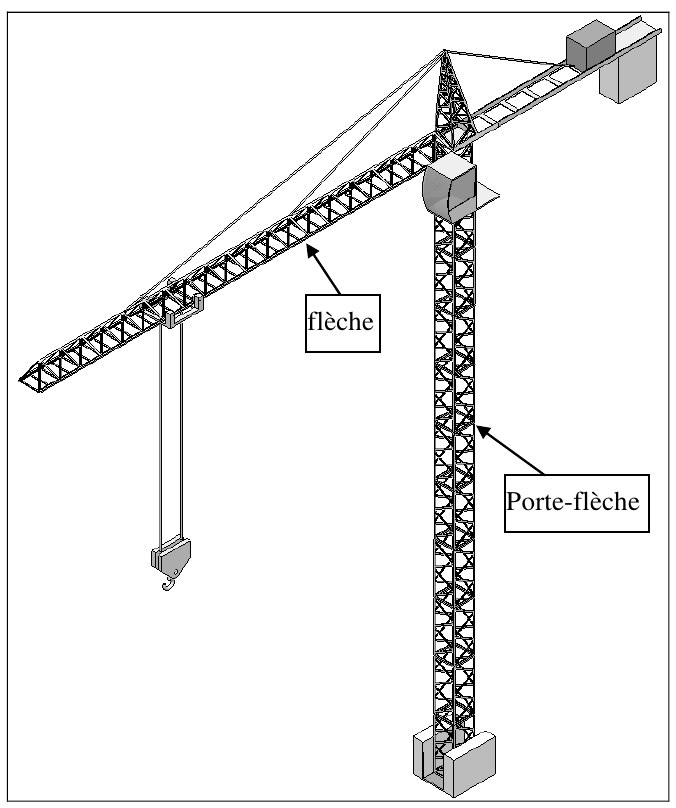
\includegraphics[width=0.7\linewidth]{img/grue0.png}
  \caption{Grue à tour}
  \label{img:grue0}
 \end{minipage}
\end{figure}

\begin{figure}[!h]
 \begin{minipage}{0.40\linewidth}
  \centering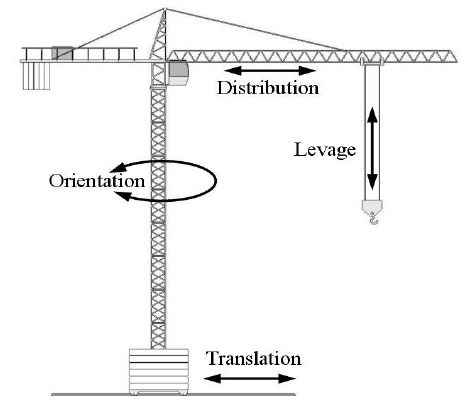
\includegraphics[width=0.9\linewidth]{img/grue1.png}
  \caption{Grue à tour}
  \label{img:grue1}
 \end{minipage}
\hfill
 \begin{minipage}{0.55\linewidth}
 Les principaux mouvements d'une grue à tour sont associés à :
\begin{itemize}
 \item la \textbf{distribution}, qui déplace le chariot le long de la flèche,
 \item le \textbf{levage}, qui déplace le crochet, suspendu par l'intermédiaire du chariot, vers le haut et vers le bas,
 \item l'\textbf{orientation}, qui fait tourner l'ensemble de l'équipement flèche de gauche à droite,
 \item la \textbf{translation}, qui déplace l'ensemble de la grue sur un rail fixé au sol.
\end{itemize}
 \end{minipage}
\end{figure}

La mise en \oe uvre de ces mouvements s'effectue en général à partir de la cabine.

Hiérarchie des contraintes :
\begin{itemize}
 \item la sécurité est la plus importante des contraintes dans la conception et l'utilisation,
 \item la productivité,
 \item la facilité de mise en \oe uvre et de transport.
\end{itemize}

Les grues modernes disposent de fonctions qui permettent d'optimiser (ou d'interdire) leur fonctionnement en fonction :
\begin{itemize}
 \item des efforts dans sa structure (valeur et position de la charge, effets dynamiques),
 \item du vent,
 \item de zones à interdire,
 \item de la présence d'autres grues.
\end{itemize}

\subsection{Étude cinématique de la grue}

On va déterminer dans cette partie la vitesse de la masse transportée par la grue.
On définit $(G_C,\overrightarrow{x_C}, \overrightarrow{y_C}, \overrightarrow{z_C})$, le repère lié au chariot (figure \ref{img:grue2}).

Hypothèses :
\begin{itemize}
 \item La charge de masse M est supposée ponctuelle au point P d'attache avec le crochet,
 \item $\overrightarrow{OG_C}=R.\overrightarrow{x_C}$ et $\overrightarrow{G_CP}=L.\overrightarrow{z_P}$,
 \item le bâti de la grue portera le numéro 0,
 \item la flèche portera le numéro 1,
 \item le chariot portera le numéro 2,
 \item le crochet portera le numéro 3.
 \end{itemize}

\begin{figure}[!h]
  \centering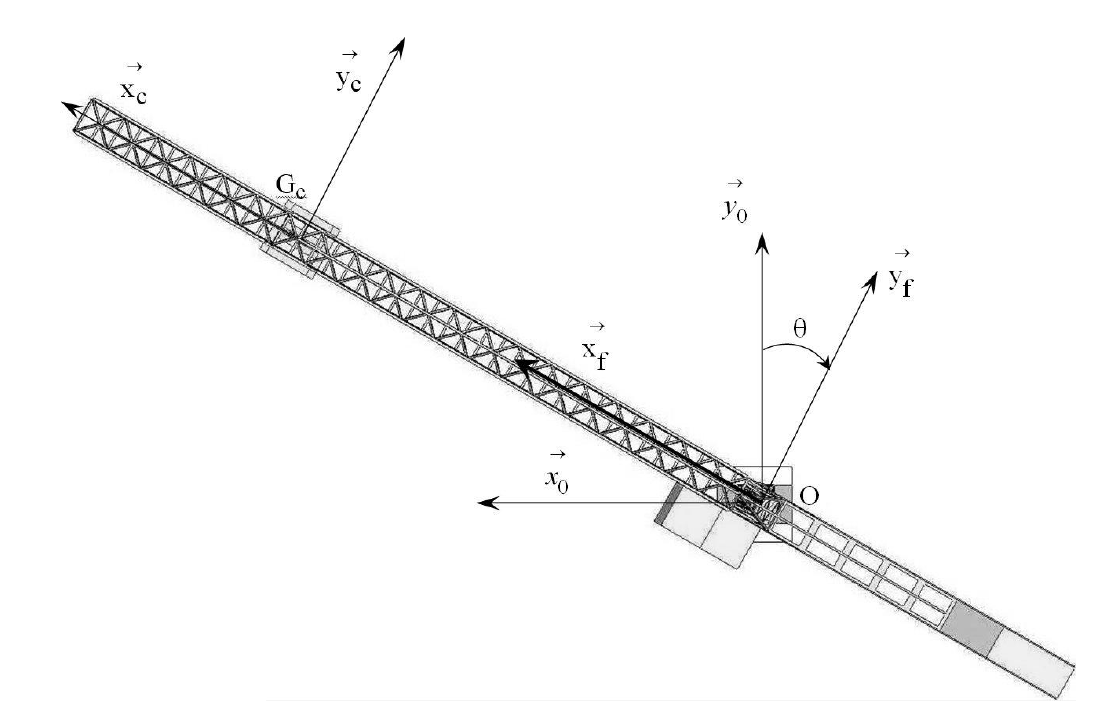
\includegraphics[width=0.8\linewidth]{img/grue2.png}
  \caption{Grue paramétrée}
  \label{img:grue2}
\end{figure}

\paragraph{Question 1:}

Déterminer la vitesse $\overrightarrow{V_{G_c \in 1/0}}$.

\paragraph{Question 2:}

Déterminer la vitesse $\overrightarrow{V_{G_c \in 2/1}}$, puis $\overrightarrow{V_{G_c \in 2/0}}$.

\paragraph{Question 3:}

Déterminer la vitesse $\overrightarrow{V_{P \in 3/2}}$, puis $\overrightarrow{V_{P \in 3/0}}$.

\paragraph{Question 4:}

Déterminer l'accélération $\overrightarrow{\Gamma_{P \in 3/0}}$.

\newpage

\section{Étude d'un poste de palettisation de bidons}

La société Agronutrition est une PME du tissu économique midi-pyrénéen. Elle conçoit, fabrique et commercialise une large gamme de compléments nutritionnels destinés à améliorer la qualité et/ou le rendement des productions végétales (grandes cultures, vigne, arboriculture, maraîchage).

L'étude se limitera à l'atelier de conditionnement des produits, aujourd'hui en partie automatisé.

\subsection{Atelier de conditionnement des produits}

\subsubsection{Présentation}

Les produits réalisés par l'entreprise Agronutrition se présentent sous forme liquide et sont élaborés et stockés dans des cuves avant d'être conditionnés dans des bidons de 5, 10, 20 ou 40 litres.

Les bidons vides sont livrés par palettes. Le conditionnement des produits consiste en un certain nombre d'opérations réalisées sur des postes spécifiques :

\begin{figure}[!h]
 \begin{minipage}{0.55\linewidth}
\begin{itemize}
 \item Poste 1 : dépalettisation des bidons vides,
 \item Poste 2 : remplissage des bidons,
 \item Poste 3 : bouchage des bidons,
 \item Poste 4 : marquage jet d'encre des bidons pour assurer leur traçabilité,
 \item Poste 5 : collage étiquette,
 \item Poste 6 : palettisation des bidons,
 \item Poste 7 : stockage des palettes pleines.
\end{itemize}
 \end{minipage}
\hfill
 \begin{minipage}{0.40\linewidth}
  \centering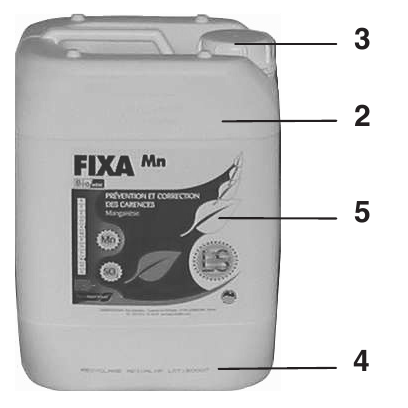
\includegraphics[width=0.5\linewidth]{img/bidon.png}
  \caption{Bidon}
  \label{img:image101}
 \end{minipage}
\end{figure}

Seules les opérations 2, 3, 4, 5 et 6 sont aujourd'hui entièrement automatisées. En particulier, la palettisation des bidons pleins au poste 6 est réalisée par un robot Kuka KR 180-2 PA dont les caractéristiques sont précisées sur la figure \ref{img:image104}.

\subsection{Analyse cinématique du robot}

\subsubsection{Objectif}

On souhaite tout d'abord s'assurer que, pour tous les conditionnements de produit, le robot pourra mettre en position le bidon le plus éloigné situé dans les coins du bord extérieur de la palette.

On s'intéressera ensuite aux particularités des mouvements du robot (dont la vocation est la palettisation) résultant de l'utilisation d'un double parallélogramme.

%\begin{figure}[!h]
%  \centering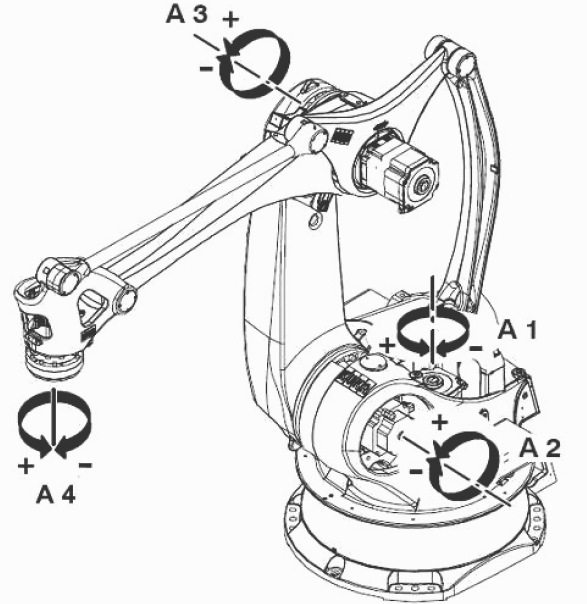
\includegraphics[width=0.5\linewidth]{img/figure11.png}
%  \caption{Mobilités du système}
%  \label{img:image11}
%\end{figure}

\subsubsection{Données}

\begin{itemize}
 \item L'espace de travail du robot est défini Figure 15, annexe 1,
 \item Les palettes sont disposées symétriquement par rapport à l'axe $\overrightarrow{O_0x0}$,
 \item On suppose que l'axe vertical de symétrie d'un bidon est confondu avec l'axe $(O_4,\overrightarrow{z_4})$ et que la face supérieure d'un bidon est située dans le plan $(\overrightarrow{x_4},\overrightarrow{z_4})$,
\end{itemize} 

 \begin{minipage}{0.5\linewidth}
\begin{itemize}
 \item $\overrightarrow{O_{10}O_4}=a.\overrightarrow{x_4}+b.\overrightarrow{z_4}$,
 \item $\overrightarrow{O_3O_{10}}=l.\overrightarrow{x_3}$,
 \item $\overrightarrow{O_2O_3}=l.\overrightarrow{x_2}$,
 \item $\overrightarrow{O_1O_2}=c.\overrightarrow{x_1}+d.\overrightarrow{z_1}$,
\end{itemize} 
 \end{minipage} \hfill
 \begin{minipage}{0.5\linewidth}
\begin{itemize}
 \item $\alpha_0=(\overrightarrow{x_0},\overrightarrow{x_1})=(\overrightarrow{y_0},\overrightarrow{y_1})$,
 \item $\theta_2=(\overrightarrow{x_1},\overrightarrow{x_2})=(\overrightarrow{z_1},\overrightarrow{z_2})$,
 \item $\theta_3=(\overrightarrow{x_1},\overrightarrow{x_3})=(\overrightarrow{z_1},\overrightarrow{z_3})$.
\end{itemize}
 \end{minipage}


\begin{figure}[!h]
  \centering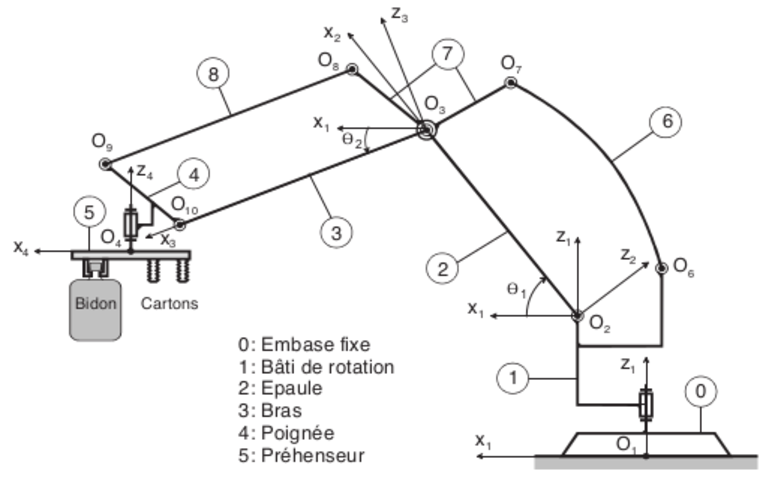
\includegraphics[width=0.7\linewidth]{img/annexe_robot}
  \caption{Dimensions du système}
  \label{img:image104}
\end{figure}


\paragraph{Question 1:} Quelle figure géométrique constitue la chaîne de fermeture géométrique $O_3O_8O_9O_{10}$ ? Que pouvez vous en déduire concernant les côtés $O_3O_8$ et $O_9O_{10}$ ? En déduire la nature du mouvement de 4 par rapport à 7.

\paragraph{Question 2:} D'après la question précédente, déterminer la nature du mouvement de 7 par rapport à 1.

\paragraph{Question 3:} En supposant les différents moteurs alimentés et en désignant par $\omega_{i}$ la vitesse angulaire correspondant à $\dot{\theta_i}$, déterminer:
\begin{enumerate}
 \item $\overrightarrow{V_{(O_4\in4/7)}}$ : vitesse de $O_4$ appartenant à 4 par rapport à 7,
 \item $\overrightarrow{V_{(O_4\in7/1)}}$ : vitesse de $O_4$ appartenant à 7 par rapport à 1,
 \item $\overrightarrow{V_{(O_4\in1/0)}}$ : vitesse de $O_4$ appartenant à 1 par rapport au sol,
 \item $\overrightarrow{V_{(O_4\in4/0)}}$ : vitesse de $O_4$ appartenant à 4 par rapport au sol.
\end{enumerate}

\paragraph{Question 4:} En déduire le vecteur accélération $\overrightarrow{\Gamma_{(O_4\in4/0)}}$, accélération de $O_4$ appartenant à 4 par rapport au sol.

\paragraph{Question 5:} Déterminer $\overrightarrow{\Omega_{4/1}}$. En déduire la nature du mouvement du poignet 4 par rapport à la pièce 1.
Ceci correspond-il à la vocation de palettisation du robot ? Quel est l'intérêt d'une telle structure par rapport à celle d'un robot 6 axes (voir figure \ref{img:image5}) ?

\paragraph{Question 6:} Déterminer si-possible les champs de vecteur vitesse et d'accélération suivants:
\begin{enumerate}
 \item mouvement de 4 par rapport à 7,
 \item mouvement de 7 par rapport à 1,
 \item mouvement de 1 par rapport au sol.
\end{enumerate}

\newpage

\section{Attelage automatique type 10L}

\begin{figure}[!h]
 \begin{minipage}{0.6\linewidth}
Pour offrir aux passagers des déplacements à très grande vitesse, la SNCF dispose de rames TGV composées chacune de 2 motrices encadrant 8 voitures.

Dans certains cas d'affluence, veille de \og grand week-end \fg ou vacances scolaires, afin de transporter un maximum de passagers, la SNCF réalise l'assemblage de 2 rames, au niveau des motrices, par le biais d'un attelage de type 10L. Cet attelage est composé de deux demi-attelages.

Au désaccouplement, il reste un demi-attelage sur chacune des motrices.
 \end{minipage}
\hfill
 \begin{minipage}{0.35\linewidth}
  \centering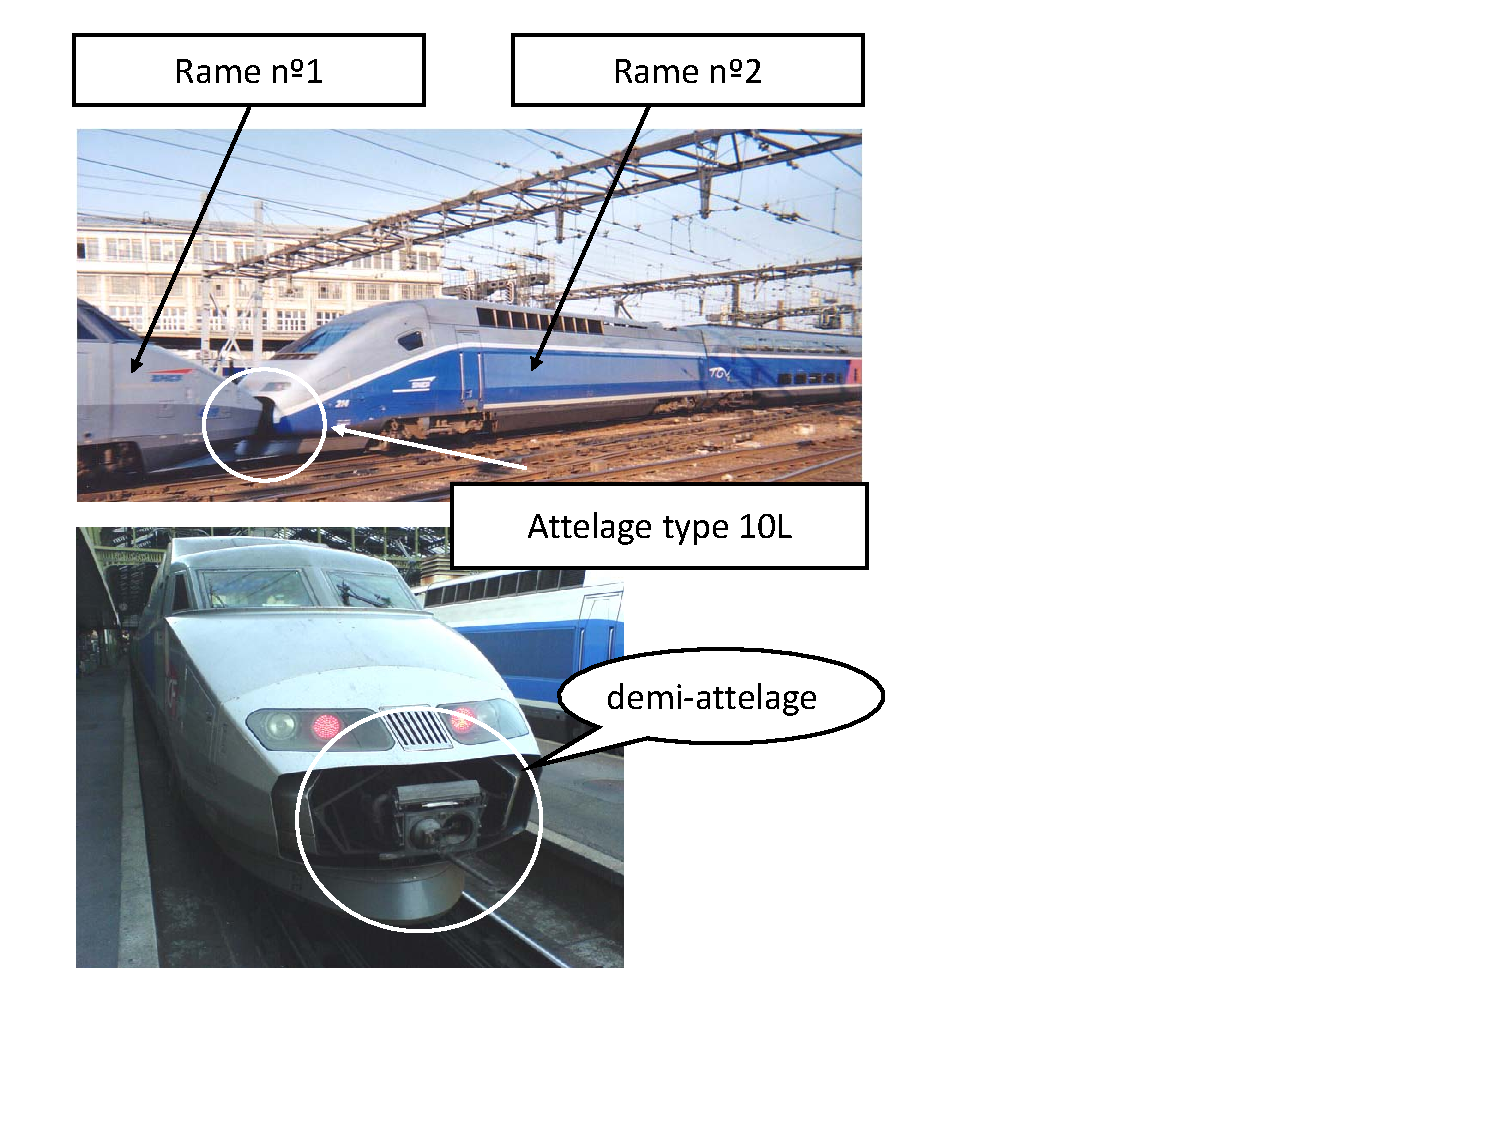
\includegraphics[width=\linewidth]{img/Image1.pdf}
  \caption{TGV et son attelage}
  \label{img:image1}
 \end{minipage}
\end{figure}

\subsection{Présentation du dispositif d'attelage SCHARFENBERG type 10L}

La société SCHARFENBERG a mis au point le dispositif d'attelage dénommé \og Attelage automatique type 10L \fg composé de deux demi-attelages comprenant chacun (voir schéma ci-dessous):
\begin{itemize}
 \item un ensemble amortisseur pour absorber les chocs en traction ou en freinage, monté en liaison rotule avec le châssis de la motrice par l'intermédiaire d'un support. Cet ensemble est maintenu horizontalement dans l'axe longitudinal de la motrice par des dispositifs de maintien,
 \item une tête d'attelage, fixée sur l'ensemble amortisseur, composée d'un coupleur électrique, d'un coupleur pneumatique et d'un coupleur mécanique (objet de l'étude).
\end{itemize}

\begin{figure}[!h]
\centering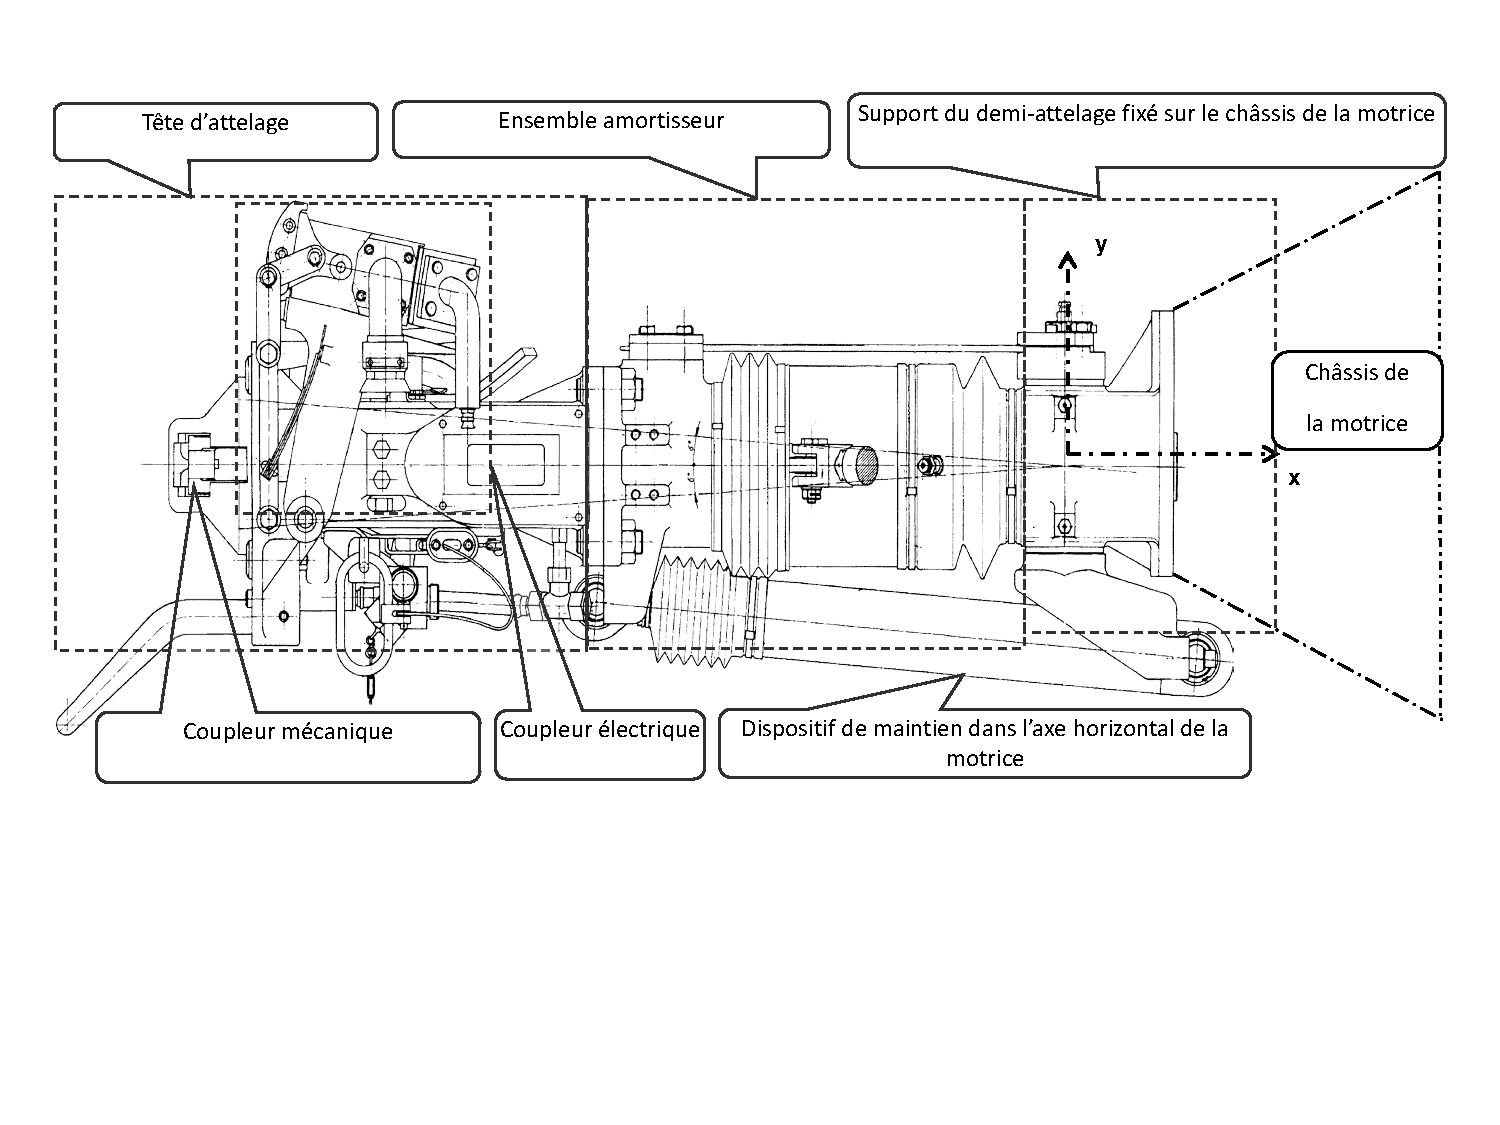
\includegraphics[width=0.75\linewidth]{img/Image2.pdf}
 \caption{Attelage du TGV}
 \label{img:image2}
\end{figure}

\subsection{Description des attelages}

\begin{figure}[!h]
 \begin{minipage}{0.5\linewidth}
\centering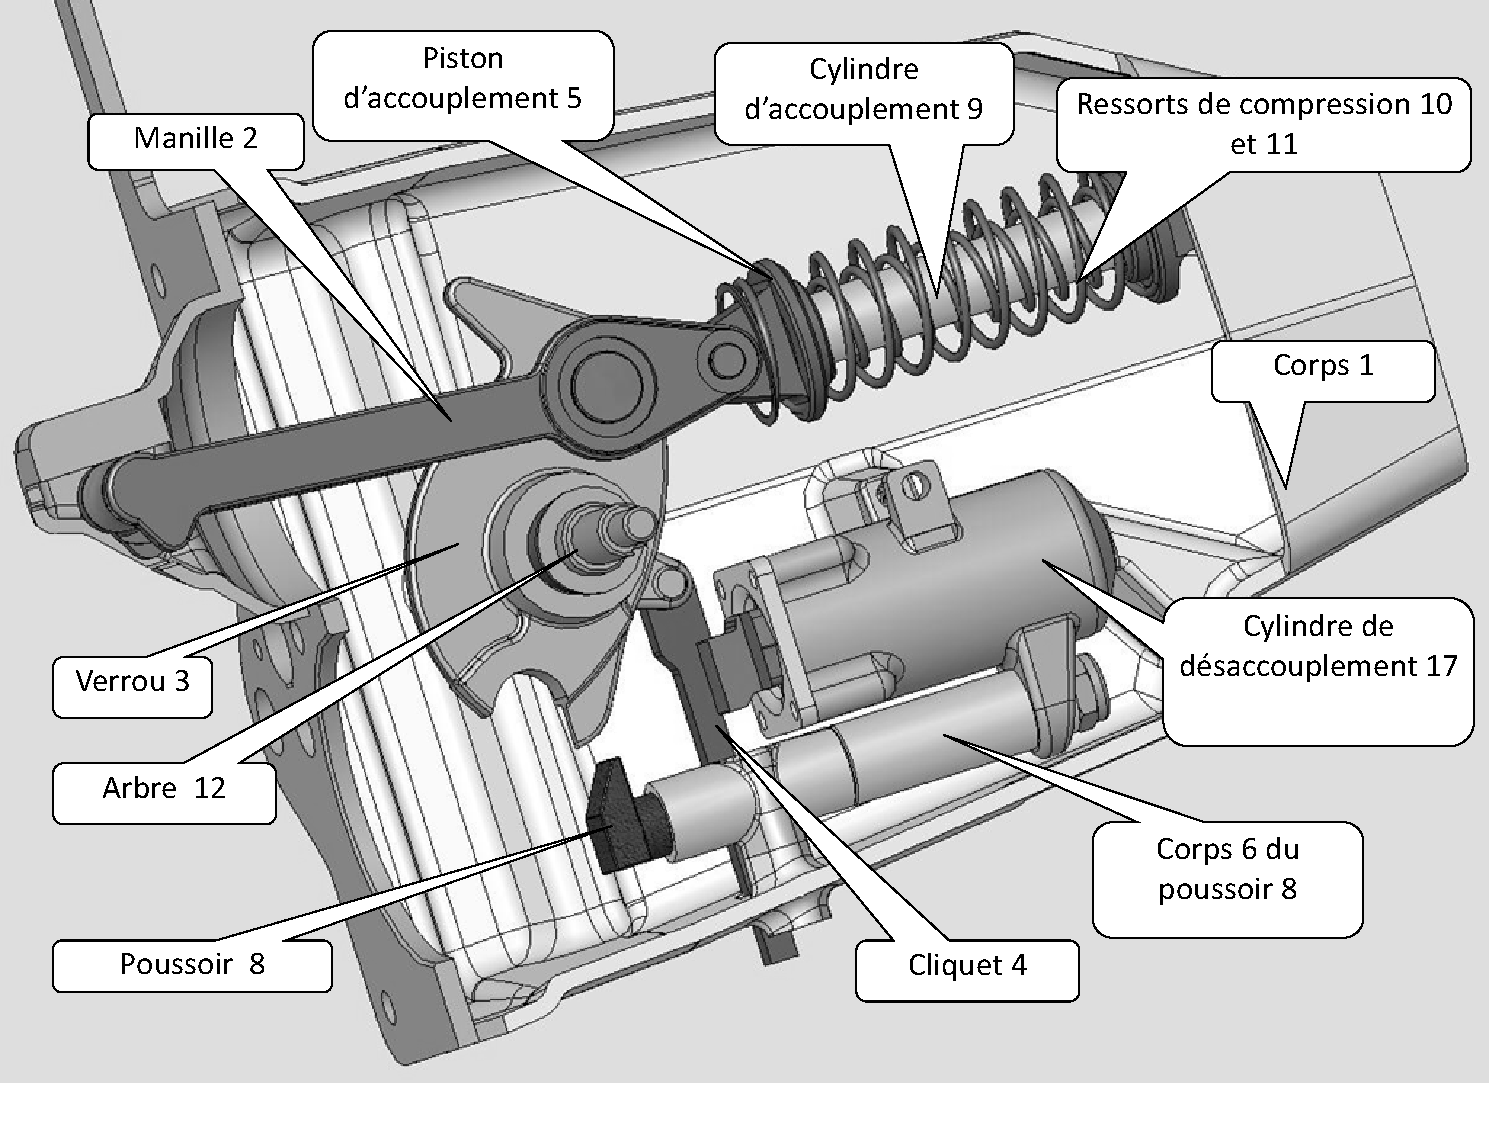
\includegraphics[width=\linewidth]{img/Image3.pdf}
 \caption{Pièces principales}
 \label{img:image3}
 \end{minipage}
\hfill
 \begin{minipage}{0.49\linewidth}
\centering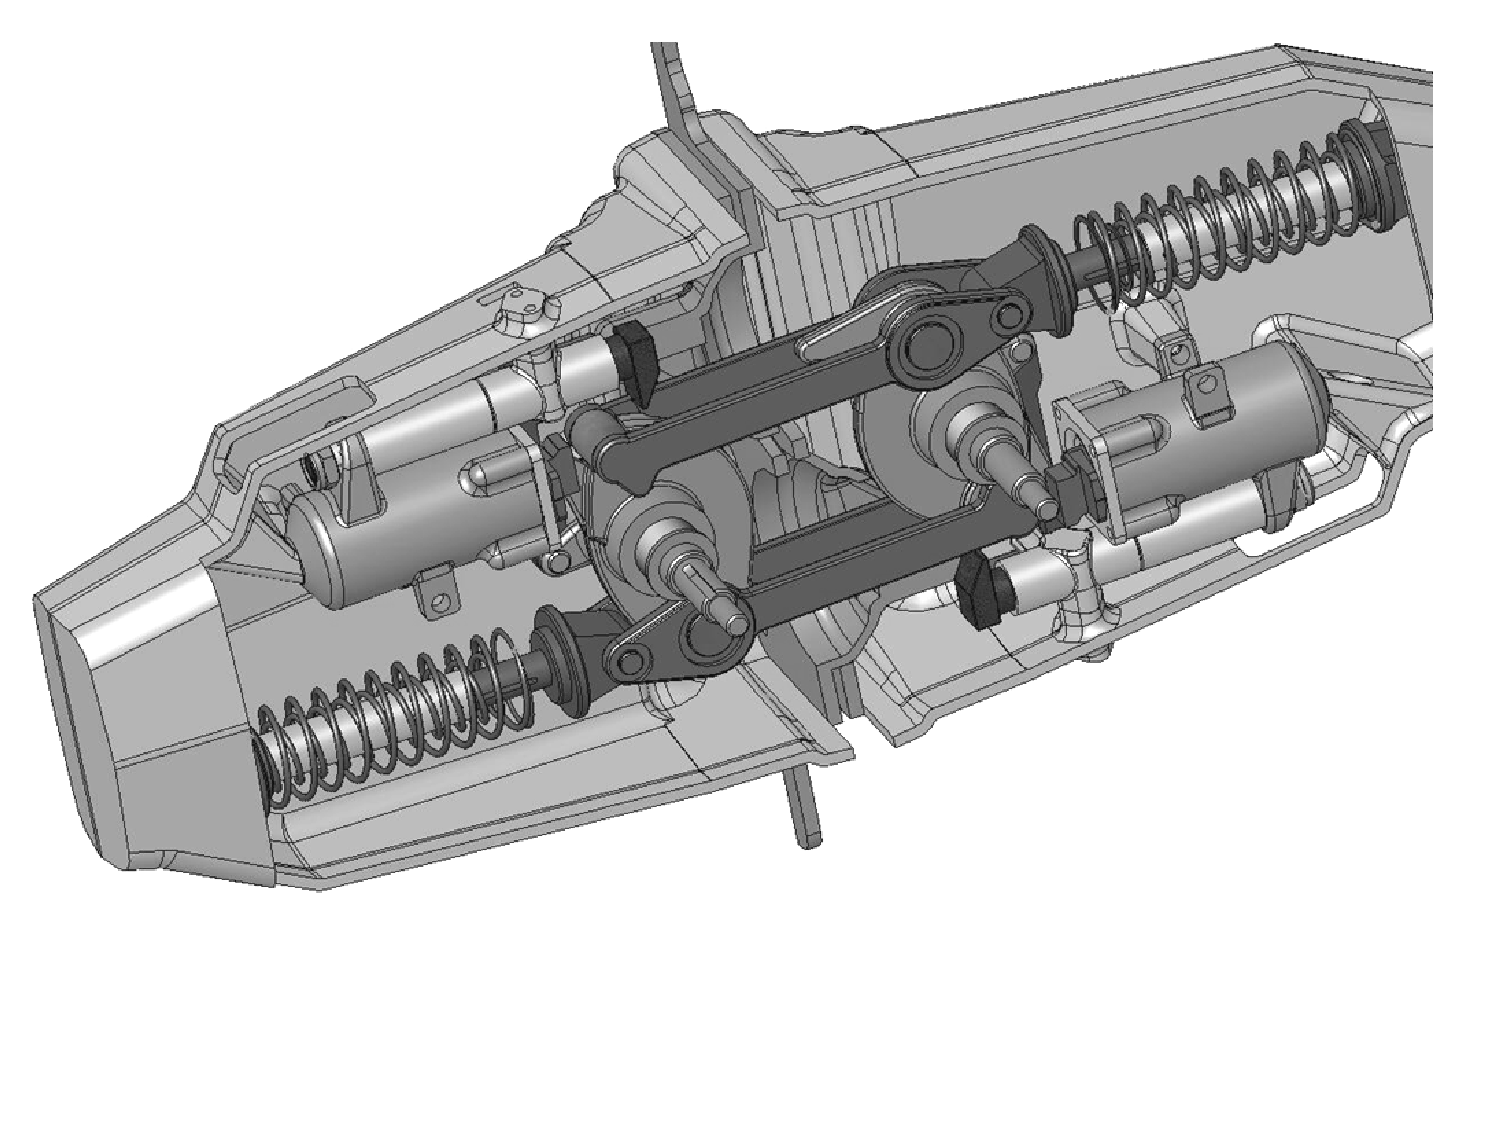
\includegraphics[width=\linewidth]{img/Image4.pdf}
 \caption{Attelages liés}
 \label{img:image4}
 \end{minipage}
\end{figure}

\subsection{Etude de cinématique graphique}

Objectif de l'étude : avant son basculement, la manille 2 glisse sur le corps 1. Le contact est direct, graissé, et dans ces conditions la vitesse maximale de glissement admise est de $1 m.s^{-1}$. Il en est de même pour le glissement du piston 5 dans le cylindre 9. L'étude qui suit propose de vérifier la conformité du mécanisme à cette obligation.

Dans une première approche, l'étude est menée pour une position donnée du mécanisme, les tracés seront réalisés sur le document réponse. Les justifications seront rédigées sur feuille de copie.

Hypothèse : pendant le glissement de la manille, on admet que la vitesse angulaire $\omega_{3/1}$ du verrou 3 est constante.

Donnée : avant le basculement de la manille, on constate que le verrou 3 tourne d'un 	angle $\theta_{3/1}$ de 20\textdegree  en 0,05 seconde.

\paragraph{Question 1:}

Calculer la vitesse de rotation angulaire moyenne $\omega_{3/1}$ et la norme du vecteur vitesse $\overrightarrow{V_{A \in 3/1}}$ sachant que OA = 85 mm.

Quel que soit le résultat obtenu à la question précédente, prendre $\|\overrightarrow{V_{A \in 3/1}}\|=0,6m.s^{-1}$.

\paragraph{Question 2:}

Montrer que $\overrightarrow{V_{A \in 2/1}}=\overrightarrow{V_{A \in 3/1}}$

Pour les questions suivantes, les tracés seront réalisés sur le document réponse DR2, figure1.

\paragraph{Question 3:}

Déterminer graphiquement la position du centre instantané de rotation \og $I_{2/1}$ \fg du mouvement de la manille 2 par rapport au corps 1. Justifier votre construction.

\paragraph{Question 4:}

Tracer $\overrightarrow{V_{A \in 2/1}}$ et déterminer graphiquement $\overrightarrow{V_{E \in 2/1}}$ par la méthode de votre choix. Justifier les étapes de votre démarche.

\paragraph{Question 5:}

Déterminer graphiquement $\overrightarrow{V_{B \in 2/1}}$. Justifier les étapes de votre démarche.

Pour les questions suivantes, les tracés seront réalisés sur le document réponse DR2, figure 2. Quel que soit le résultat obtenu à la question précédente, prendre le support de $\overrightarrow{V_{B \in 2/1}}$ indiqué sur la figure 2 et prendre $\|\overrightarrow{V_{B \in 2/1}}\|=0,65m.s^{-1}$.

\paragraph{Question 6:}

Définir les mouvements suivants :
\begin{itemize}
 \item manille 2 par rapport au piston 5, Mvt 2/5,
 \item piston 5 par rapport au cylindre 9, Mvt 5/9,
 \item cylindre 9 par rapport au corps 1, Mvt 9/1.
\end{itemize}

\paragraph{Question 7:}

Justifier que $\overrightarrow{V_{B \in 2/5}}=0$.

\paragraph{Question 8:}

Justifier et tracer le support de $\overrightarrow{V_{B \in 5/9}}$ et le support de $\overrightarrow{V_{B \in 9/1}}$.

\paragraph{Question 9:}

Ecrire la relation de composition des vecteurs vitesses au point B.

\paragraph{Question 10:}

Traduire graphiquement cette relation et en déduire la vitesse de glissement du piston 5 dans le cylindre 9 : $\overrightarrow{V_{B \in 5/9}}$.

\paragraph{Question 11:}

A l'aide des résultats obtenus aux questions 4 et 10, conclure quant au respect du cahier des charges relatif aux vitesses de glissement entre 2 et 1 et entre 5 et 9, dans la position particulière de la figure.

%\paragraph{Question 12:}
%
%Une étude plus complète à l'aide d'un logiciel de simulation a permis d'obtenir les courbes de variation de la norme des vecteurs vitesses $\overrightarrow{V_{E \in 2/1}}$ et $\overrightarrow{V_{B \in 5/9}}$ en fonction de l'angle $\theta_{3/1}$ du verrou 3, voir document DT7.
%Relever la valeur maximale de la norme des deux vecteurs vitesses. 
%Les vitesses de glissement entre 2 et 1 d'une part et entre 5 et 9 d'autre part, tout au long du mouvement de guidage de la manille, sont-elles conformes aux exigences du cahier des charges? Justifier votre réponse.

\begin{figure}[!h]
\centering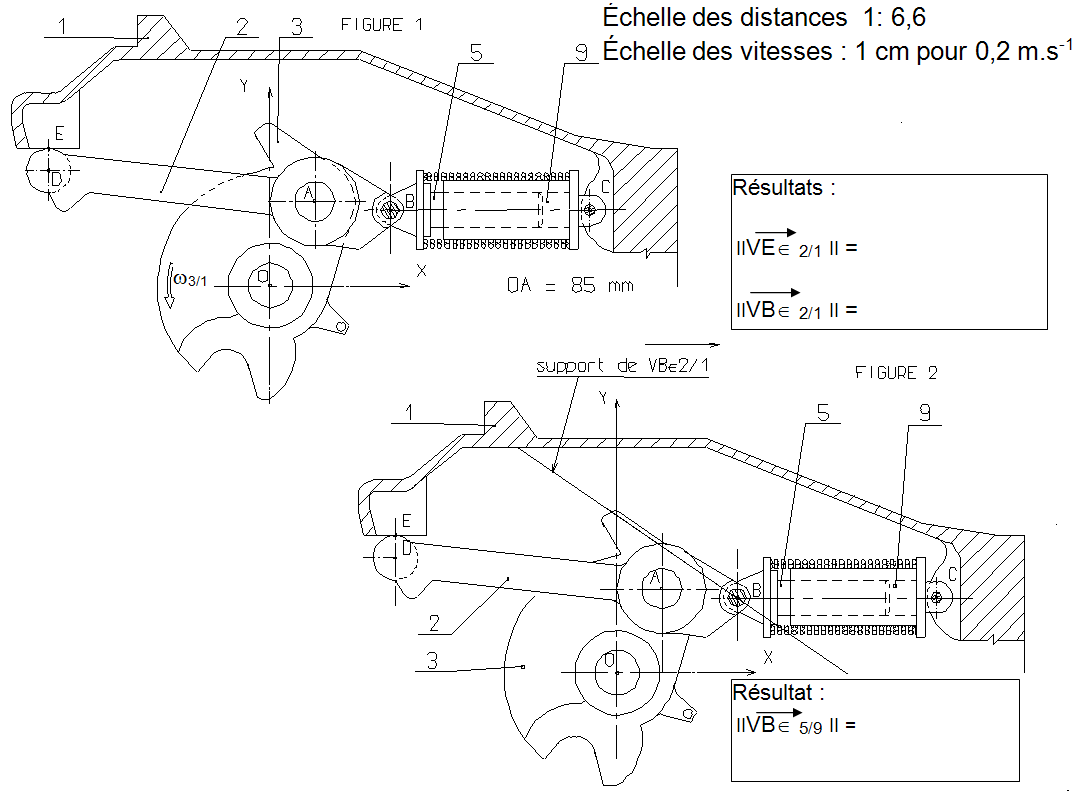
\includegraphics[width=1.2\linewidth,angle=90]{img/cin_graph.png}
 \caption{Document réponse cinématique graphique}
 \label{img:image105}
\end{figure}

\newpage

~\

\newpage

\section{Pompe doseuse}

\subsection{Présentation}

Ce type de pompe utilise un piston coulissant de manière étanche dans un cylindre pour repousser un fluide, admis précédemment dans le cylindre par l'intermédiaire d'un clapet, d'une soupape ou d'une lumière, grâce à l'aspiration provoquée par le recul du piston.

Les performances sont élevées :
\begin{itemize}
 \item pression de plusieurs milliers de bar, notamment pour le découpage jet d'eau,
 \item Débit jusqu'à 500 litres/min,
 \item Rendement > 0,951.
\end{itemize}

~\

Il existe différents montages mécaniques dont :
\begin{itemize}
 \item \textbf{Pompe à pistons axiaux}

 Pistons situés parallèlement à l'axe de transmission. Ils fonctionnent grâce à :
\begin{itemize}
 \item une glace sur laquelle glissent les patins situés en pied de pistons ;
 \item un barillet dans lequel sont logés les pistons.
\end{itemize}
Certaines pompes peuvent fonctionner avec des solutions aqueuses, voire à l'eau pure.
 
 \item \textbf{Pompe à pistons radiaux}

Les patins des pistons glissent sur un excentrique ou sur une came dont le nombre de lobes est différent (de un) au nombre de pistons. Les pistons sont munis de clapets d'aspiration et de refoulement. Souvent, pour des raisons de régularité de flux, le nombre de pistons est impair (somme de sinusoïdes régulièrement déphasées).
Article détaillé : Pompe à pistons radiaux.
\end{itemize}

\subsection{Etude de cinématique graphique}

\paragraph{Question 1:}

Réaliser le schéma cinématique de la pompe et le paramétrer.

\paragraph{Question 2:}

La vitesse de rotation du moteur est de $3000 tr.min^{-1}$, la vis a un seul filet et son pas est de 4mm. Déterminer la vitesse instantanée de sortie du piston.

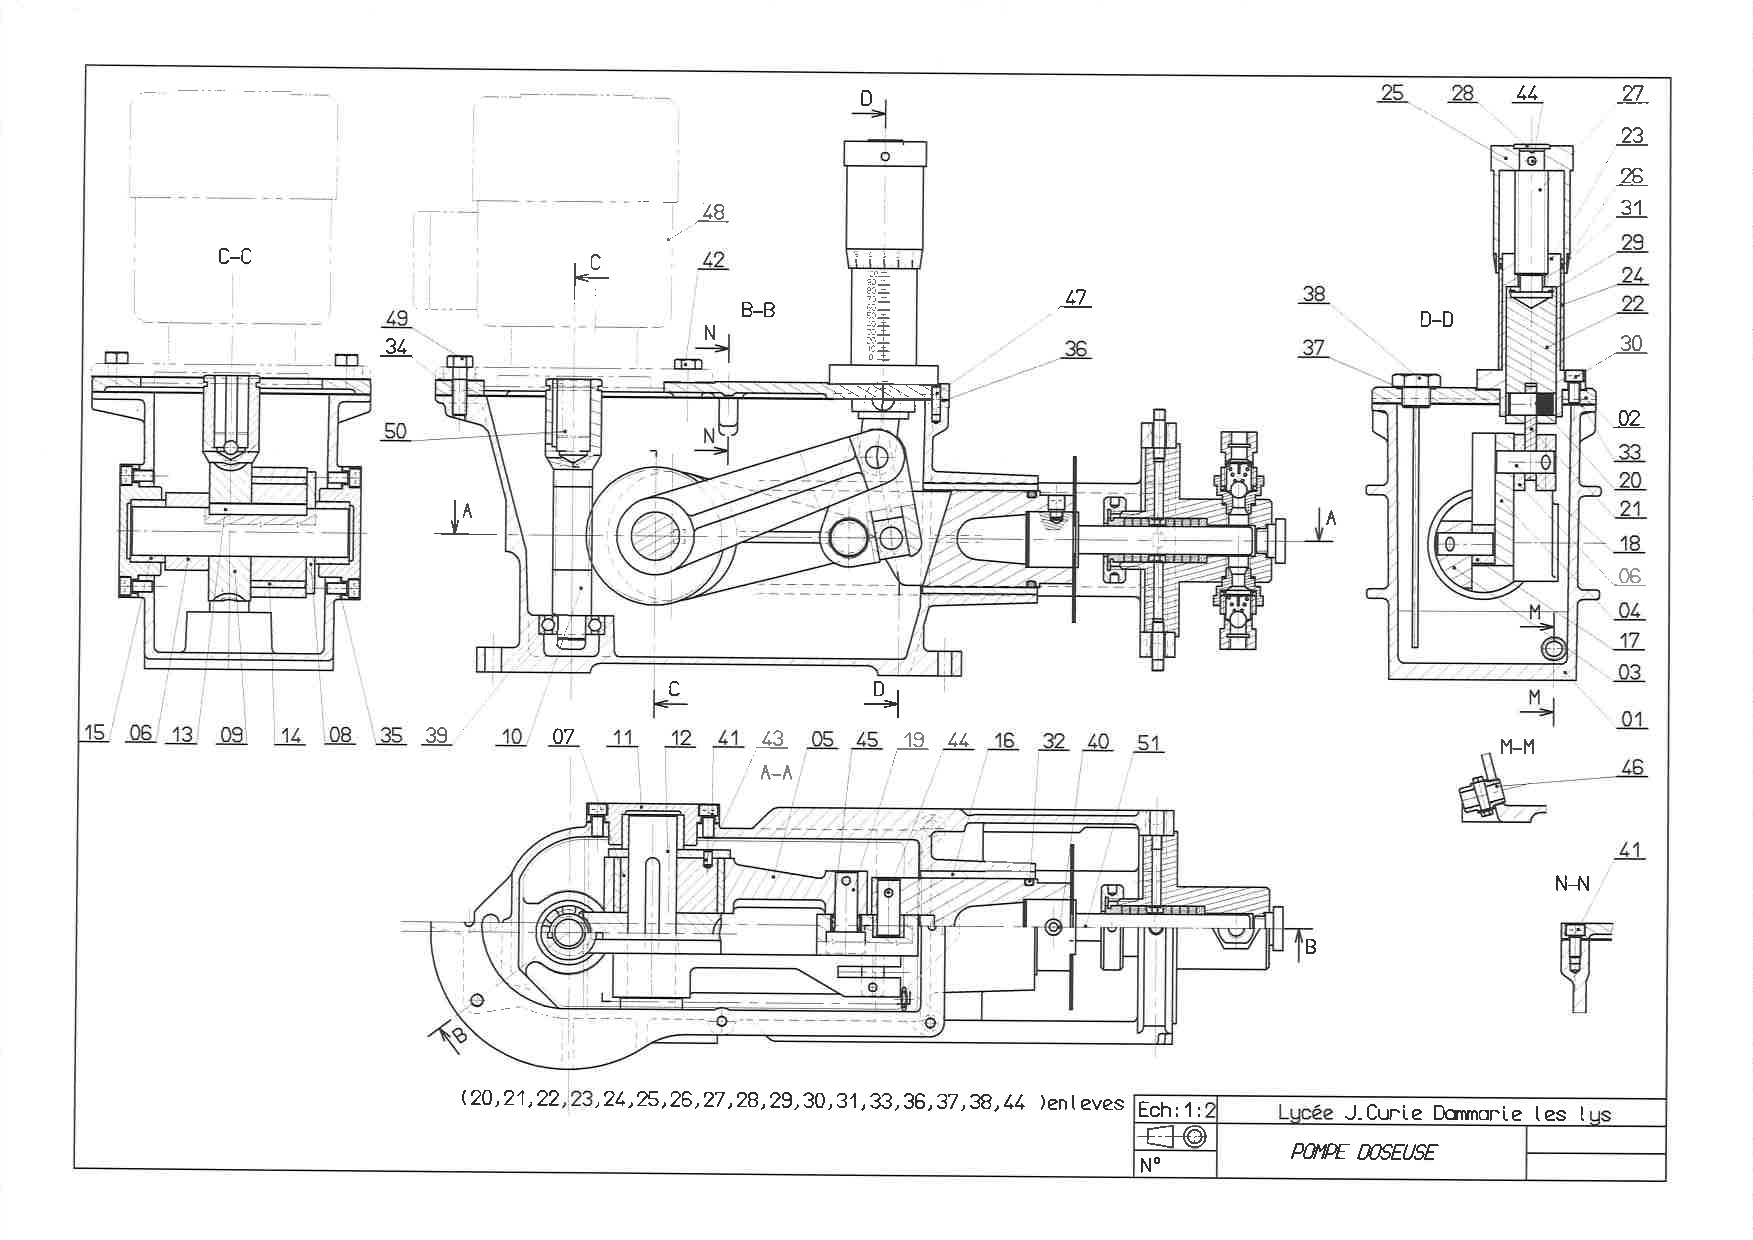
\includepdf[pages={1},landscape]{img/Pompe.pdf} 

\clearpage

\ifdef{\public}{\end{document}}{}

\pagestyle{correction}

\newpage

\section{Correction}

\subsection{Grue à tour}

\paragraph{Question 1:} 

$\overrightarrow{V_{G_c\in 1/0}}=\overrightarrow{V_{O\in 1/0}}+\overrightarrow{G_cO}\wedge \overrightarrow{\Omega_{1/0}}$

$\overrightarrow{V_{G_c\in 1/0}}=-R.\overrightarrow{x_C}\wedge \omega_{1/0}.\overrightarrow{z_c}=R.\omega_{1/0}.\overrightarrow{y_c}$

\paragraph{Question 2:} 

$\overrightarrow{V_{G_c\in 2/1}}=\dot{R}.\overrightarrow{x_c}$

$\overrightarrow{V_{G_c\in 2/0}}=\dot{R}.\overrightarrow{x_c}+R.\omega_{1/0}.\overrightarrow{y_c}$

\paragraph{Question 3:} 

$\overrightarrow{V_{P\in 3/2}}=\dot{L}.\overrightarrow{z_p}$

$\overrightarrow{V_{P\in 3/0}}=\overrightarrow{V_{P\in 3/2}}+\overrightarrow{V_{P\in 2/0}}$

$\overrightarrow{V_{P\in 3/0}}=\overrightarrow{V_{P\in 3/2}}+\overrightarrow{V_{G_c\in 2/0}}+\overrightarrow{PG_c}\wedge \overrightarrow{\Omega_{2/0}}$

$\overrightarrow{V_{P\in 3/0}}=\dot{L}.\overrightarrow{z_p}+\dot{R}.\overrightarrow{x_c}+R.\omega_{1/0}.\overrightarrow{y_c}-L.\overrightarrow{z_p}\wedge \Omega_{1/0}.\overrightarrow{z_p}$

$\overrightarrow{V_{P\in 3/0}}=\dot{L}.\overrightarrow{z_p}+\dot{R}.\overrightarrow{x_c}+R.\omega_{1/0}.\overrightarrow{y_c}$

\paragraph{Question 4:} 

$\overrightarrow{\Gamma_{P\in 3/0}}=\ddot{L}.\overrightarrow{z_p}+\ddot{R}.\overrightarrow{x_c}+\dot{R}.\omega_{1/0}.\overrightarrow{y_c}+(\dot{R}.\omega_{1/0}+R.\dot{\omega}_{1/0}).\overrightarrow{y_c}-R.\omega_{1/0}.\omega_{1/0}.\overrightarrow{x_c}$

$\overrightarrow{\Gamma_{P\in 3/0}}=(\ddot{R}-R.\omega_{1/0}^2).\overrightarrow{x_c}+(2.\dot{R}.\omega_{1/0}+R.\dot{\omega}_{1/0}).\overrightarrow{y_c}+\ddot{L}.\overrightarrow{z_p}$

\subsection{Poste de palettisation}

\paragraph{Question 1:} Quelle figure géométrique constitue la chaîne de fermeture géométrique $O_3O_8O_9O_{10}$ ? Que pouvez vous en déduire concernant les côtés $O_3O_8$ et $O_9O_{10}$ ? En déduire la nature du mouvement de 4 par rapport à 7.

Cette figure géométrique est un parallélogramme, cela signifie que $O_3O_8$ et $O_9O_{10}$ sont parallèles. Le mouvement de 4 par rapport à 7 est alors une translation.

\paragraph{Question 2:} Le mouvement de 7 par rapport à 1 est une translation pour la même raison.

\paragraph{Question 3:} 

$\overrightarrow{V_{O_{4}\in 4/7}}=\overrightarrow{V_{O_{10}\in 4/7}}=\overrightarrow{V_{O_{10}\in 3/7}}$

$\overrightarrow{V_{O_{10}\in 4/7}}=\overrightarrow{V_{O_{3}\in 3/7}}+\overrightarrow{O_{10}O_{3}}\wedge \overrightarrow{\Omega_{3/7}}$

$\overrightarrow{V_{O_{10}\in 4/7}}=-l.\overrightarrow{x_3}\wedge \omega_2.\overrightarrow{y_3}=-l.\omega_2.\overrightarrow{z_3}$

~\

$\overrightarrow{V_{O_{4}\in 7/1}}=\overrightarrow{V_{O_{3}\in 7/1}}=\overrightarrow{V_{O_{3}\in 2/1}}$

$\overrightarrow{V_{O_{3}\in 7/1}}=\overrightarrow{V_{O_{2}\in 2/1}}+\overrightarrow{O_{3}O_{2}}\wedge \overrightarrow{\Omega_{2/1}}$

$\overrightarrow{V_{O_{3}\in 7/1}}=-l.\overrightarrow{x_2}\wedge \omega_1.\overrightarrow{y_2}=-l.\omega_1.\overrightarrow{z_2}$

~\

$\overrightarrow{V_{O_{4}\in 1/0}}=\overrightarrow{V_{O_{1}\in 1/0}}+\overrightarrow{O_{4}O_{1}}\wedge \overrightarrow{\Omega_{1/0}}$

$\overrightarrow{V_{O_{4}\in 1/0}}=(\overrightarrow{O_{4}O_{10}}+\overrightarrow{O_{10}O_{3}}+\overrightarrow{O_{3}O_{2}}+\overrightarrow{O_{2}O_{1}})\wedge \overrightarrow{\Omega_{1/0}}$

$\overrightarrow{V_{O_{4}\in 1/0}}=(-a.\overrightarrow{x_4}-b.\overrightarrow{z_4}-l.\overrightarrow{x_3}-l.\overrightarrow{x_2}-c.\overrightarrow{x_1}-d.\overrightarrow{z_1})\wedge \omega_{0}.\overrightarrow{z_1}$

$\overrightarrow{V_{O_{4}\in 1/0}}=\left[a+c+l(cos\theta_1+cos\theta_2)\right].\omega_{0}.\overrightarrow{y_1}$

~\

$\overrightarrow{V_{O_{4}\in 4/0}}=-l.\omega_2.\overrightarrow{z_3}-l.\omega_1.\overrightarrow{z_2}+\left[a+c+l(cos\theta_1+cos\theta_2)\right].\omega_{0}.\overrightarrow{y_1}$

\paragraph{Question 4:}

$\overrightarrow{\Gamma_{O_{4}\in 4/0}}=-l.\dot{\omega}_2.\overrightarrow{z_3}-l.\omega_2.\left[\dfrac{d\overrightarrow{z_3}}{dt}\right]_{R_0}-l.\dot{\omega}_1.\overrightarrow{z_2}-l.\omega_1.\left[\dfrac{d\overrightarrow{z_2}}{dt}\right]_{R_0}+\left[l(-\omega_1.sin\theta_1-\omega_2.sin\theta_2)\right].\omega_{0}.\overrightarrow{y_1}$

$+\left[a+c+l(cos\theta_1+cos\theta_2)\right].\left(\dot{\omega}_{0}.\overrightarrow{y_1}+\omega_{0}.\left[\dfrac{d\overrightarrow{y_1}}{dt}\right]_{R_0}\right)$ 

$\left[\dfrac{d\overrightarrow{z_3}}{dt}\right]_{R_0}=\omega_2.\overrightarrow{x_3}+\omega_0.sin\theta_2.\overrightarrow{y_1}$

$\left[\dfrac{d\overrightarrow{z_2}}{dt}\right]_{R_0}=\omega_1.\overrightarrow{x_2}+\omega_0.sin\theta_1.\overrightarrow{y_1}$

$\left[\dfrac{d\overrightarrow{y_1}}{dt}\right]_{R_0}=-\omega_0.\overrightarrow{x_1}$

$\overrightarrow{\Gamma_{O_{4}\in 4/0}}=-l.\dot{\omega}_2.\overrightarrow{z_3}-l.\omega_2.\left(\omega_2.\overrightarrow{x_3}+\omega_0.sin\theta_2.\overrightarrow{y_1}\right)-l.\dot{\omega}_1.\overrightarrow{z_2}-l.\omega_1.\left(\omega_1.\overrightarrow{x_2}+\omega_0.sin\theta_1.\overrightarrow{y_1}\right)+\left[l(-\omega_1.sin\theta_1-\omega_2.sin\theta_2)\right].\omega_{0}.\overrightarrow{y_1}+\left[a+c+l(cos\theta_1+cos\theta_2)\right].\left(\dot{\omega}_{0}.\overrightarrow{y_1}-\omega_0^2.\overrightarrow{x_1}\right)$

~\

$\overrightarrow{\Gamma_{O_{4}\in 4/0}}=-\left[a+c+l(cos\theta_1+cos\theta_2)\right].\omega_0^2.\overrightarrow{x_1}-l.\omega_1^2.\overrightarrow{x_2}-l.\omega_2^2.\overrightarrow{x_3}$

$+\left(-l.\omega_2.\omega_0.sin\theta_2-l.\omega_1.\omega_0.sin\theta_1+\left[l(-\omega_1.sin\theta_1-\omega_2.sin\theta_2)\right].\omega_{0}+\left[a+c+l(cos\theta_1+cos\theta_2)\right].\dot{\omega}_{0}\right).\overrightarrow{y_1}-l.\dot{\omega}_1.\overrightarrow{z_2}-l.\dot{\omega}_2.\overrightarrow{z_3}$

~\

$\overrightarrow{\Gamma_{O_{4}\in 4/0}}=-\left[a+c+l(cos\theta_1+cos\theta_2)\right].\omega_0^2.\overrightarrow{x_1}-l.\omega_1^2.\overrightarrow{x_2}-l.\omega_2^2.\overrightarrow{x_3}$

$+.\left(-2.l.\omega_2.\omega_0.sin\theta_2-2.l.\omega_1.\omega_0.sin\theta_1+\left[a+c+l(cos\theta_1+cos\theta_2)\right].\dot{\omega}_{0}\right).\overrightarrow{y_1}-l.\dot{\omega}_1.\overrightarrow{z_2}-l.\dot{\omega}_2.\overrightarrow{z_3}$


\paragraph{Question 5:} $\overrightarrow{\Omega_{4/1}}=\overrightarrow{0}$, donc le mouvement est une translation ce qui convient pour la manipulation de bidons qui ne doivent pas être renversés.

\paragraph{Question 6:}

\begin{center}
 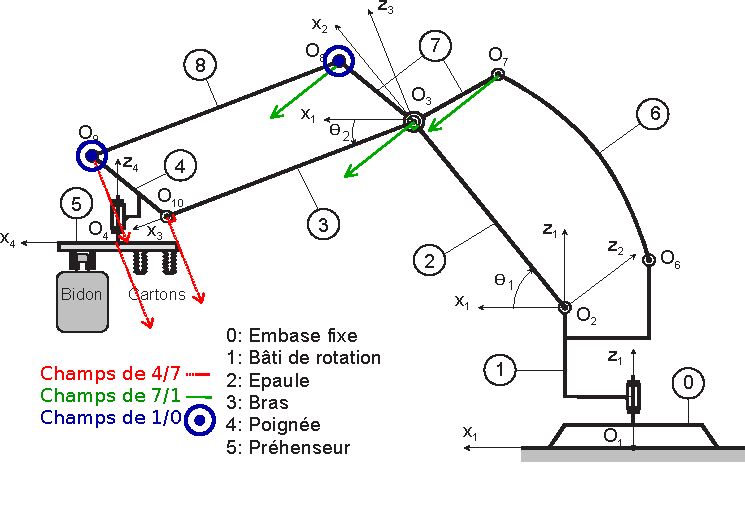
\includegraphics[width=0.8\linewidth]{img/annexe_robot_cor}
\end{center}

\newpage

\subsection{Attelage TGV}

\begin{center}
 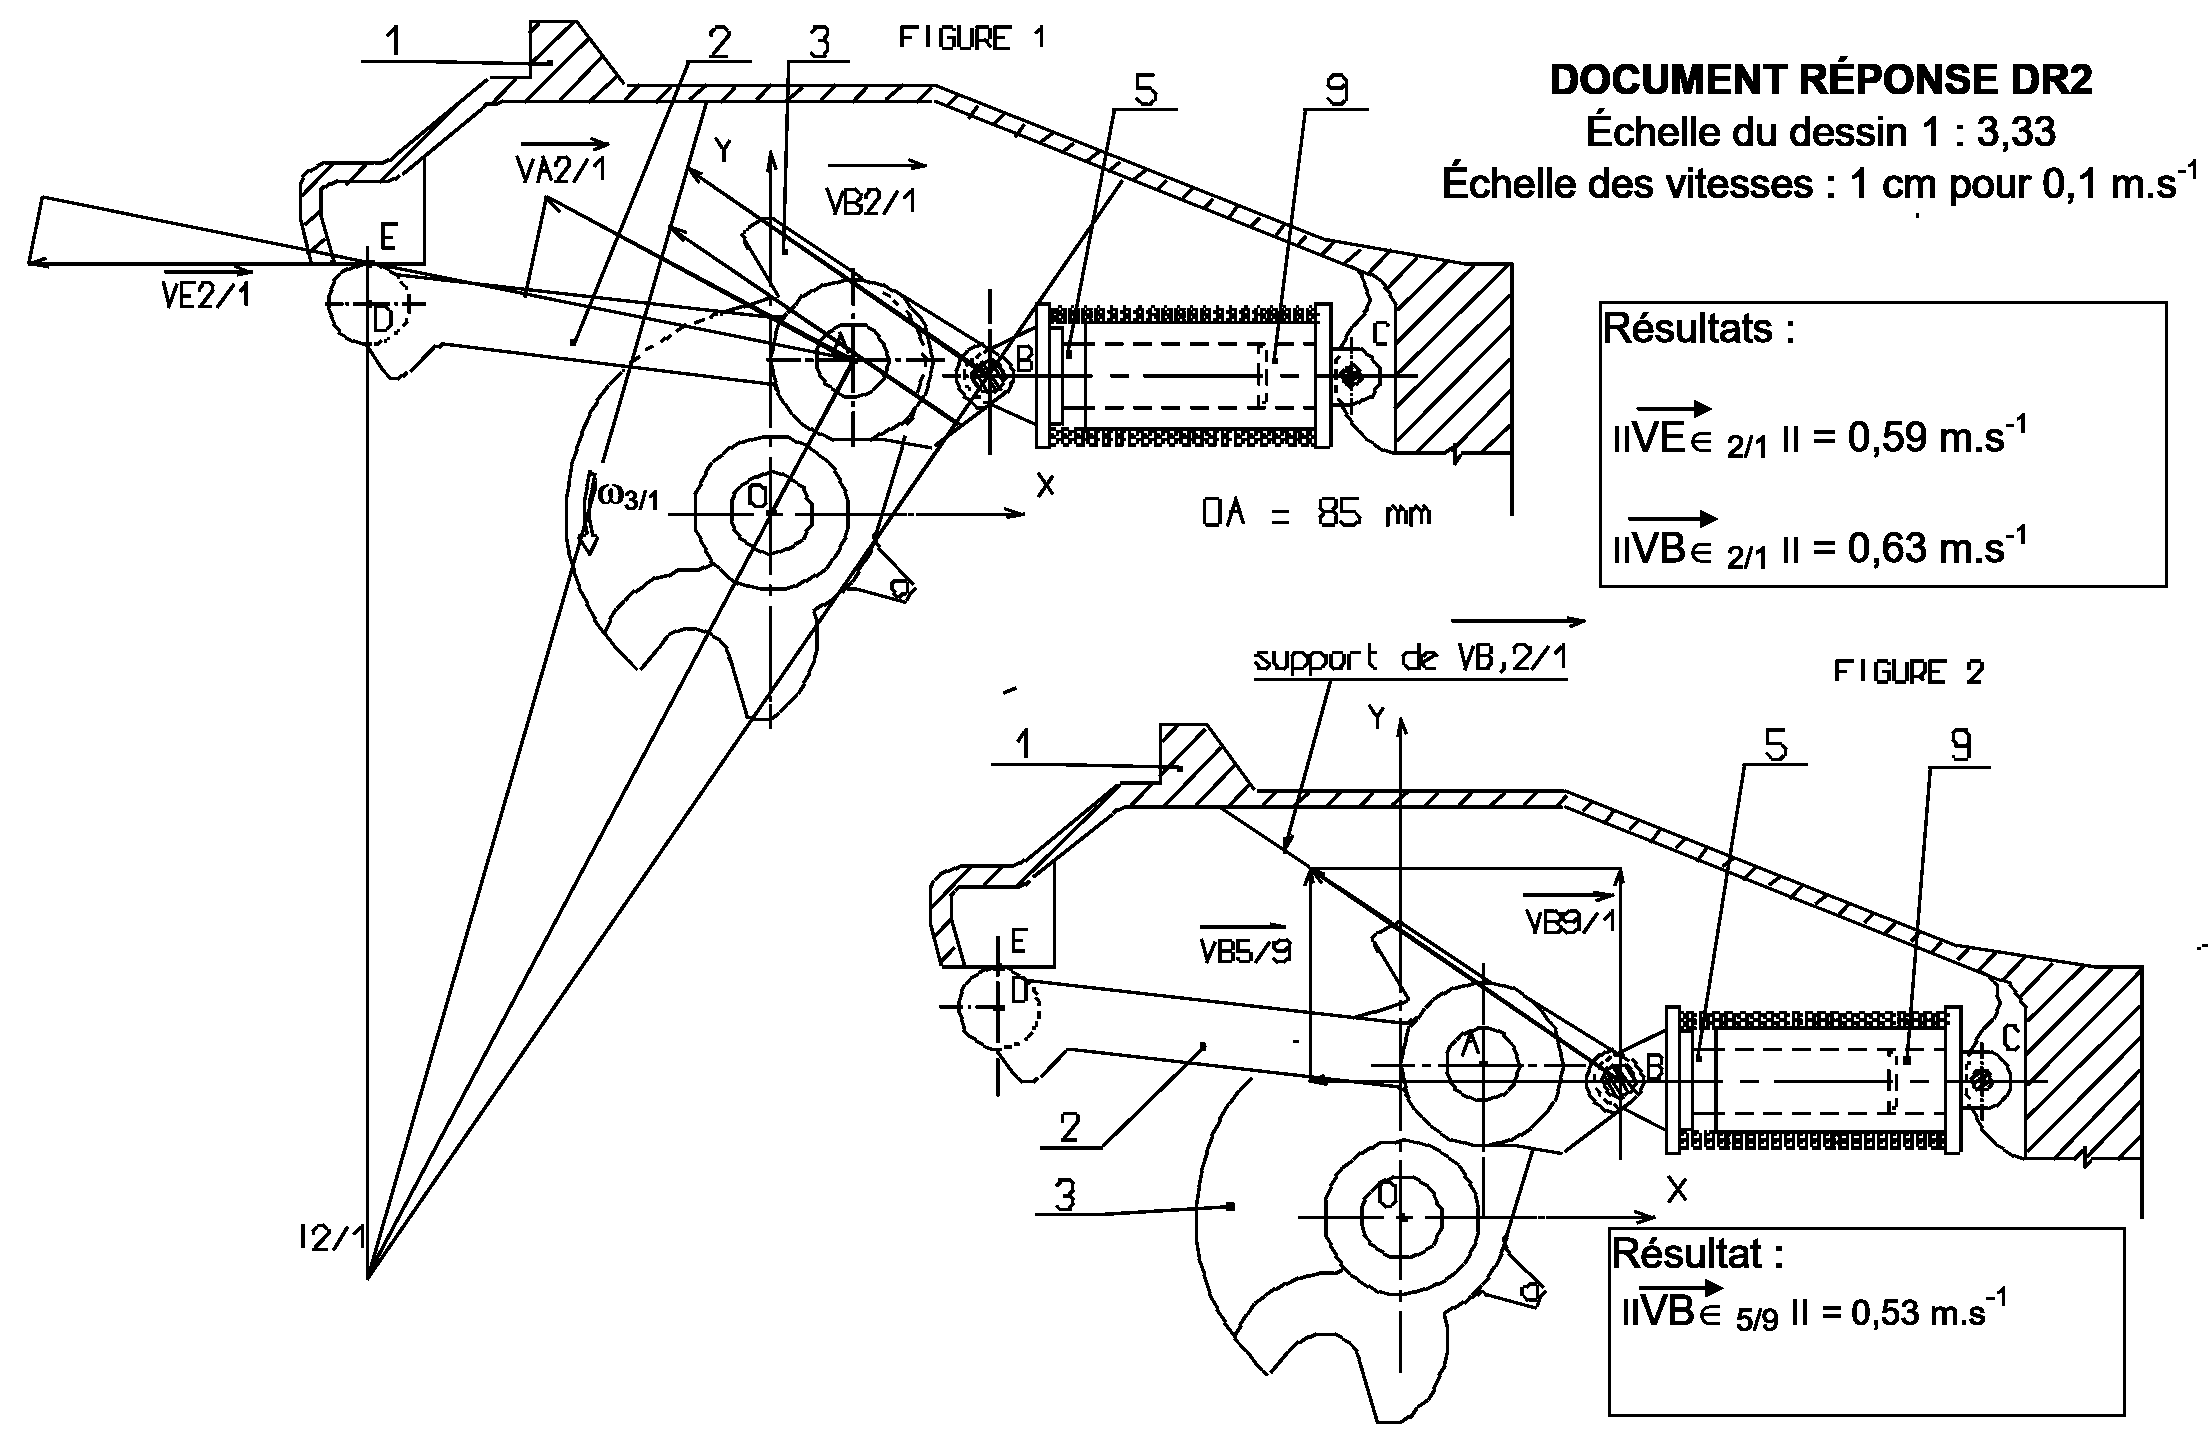
\includegraphics[width=0.8\linewidth]{img/correction_tgv}
\end{center}

\newpage

\subsection{Pompe doseuse}

\paragraph{Question 1:}

\begin{figure}[!h]
\centering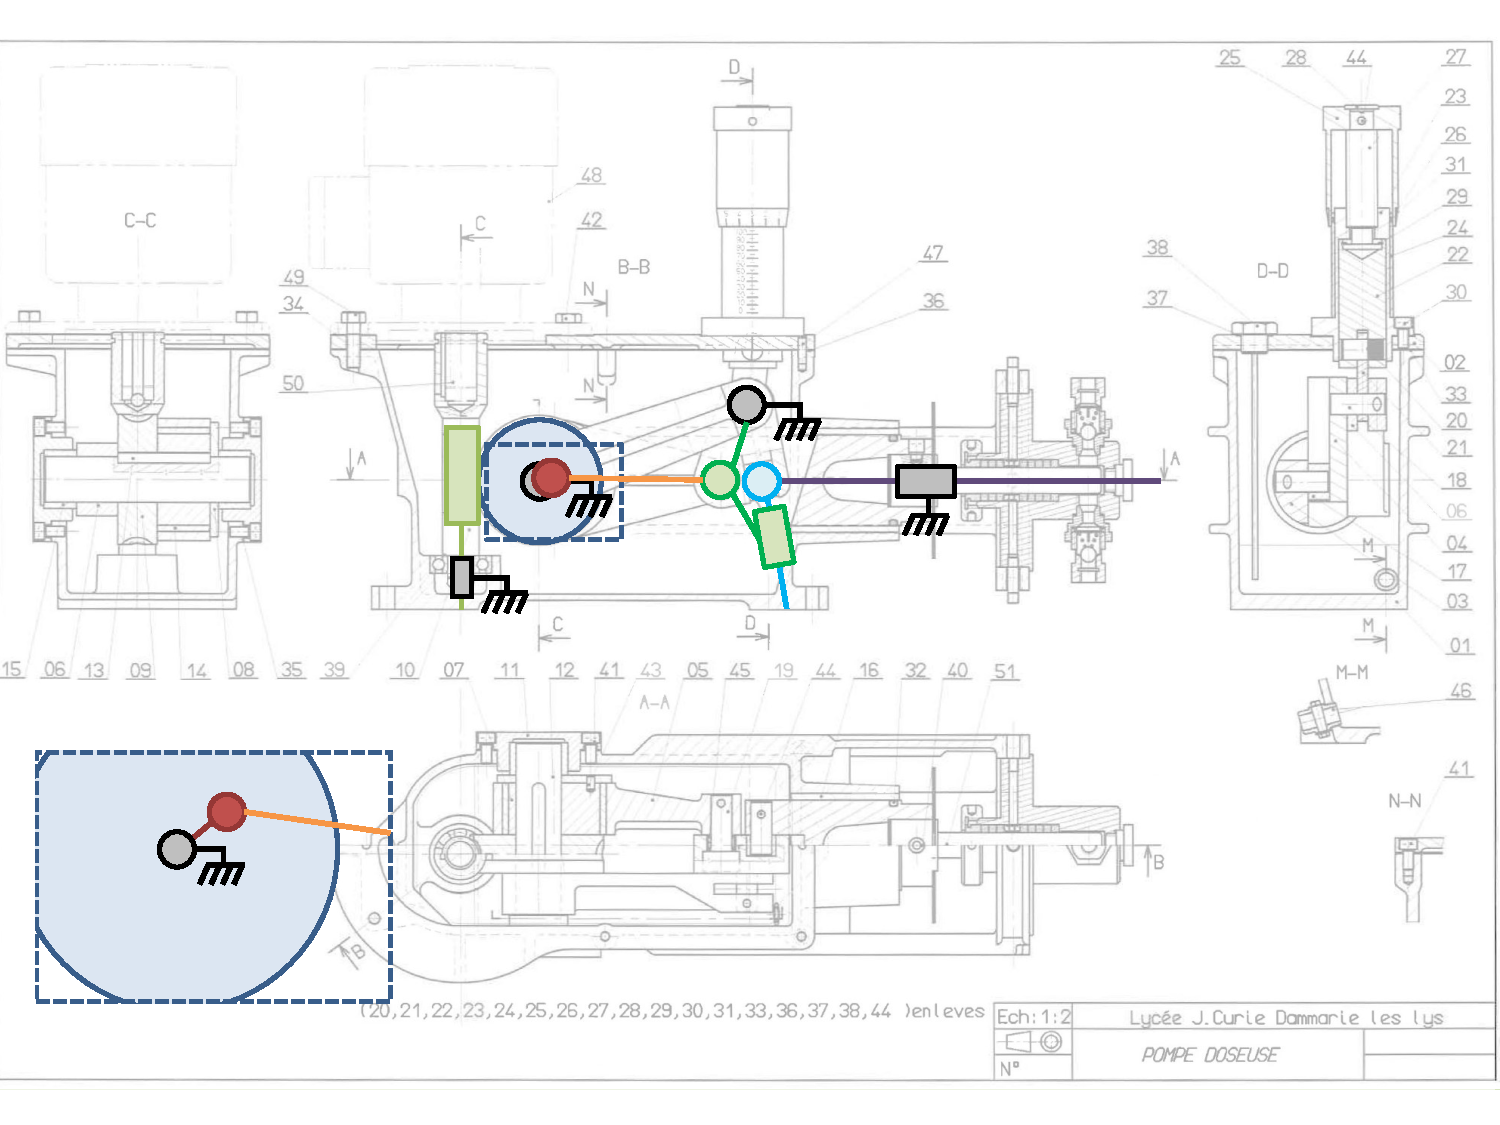
\includegraphics[width=0.8\linewidth]{img/pompe_cin.pdf}
\end{figure}

\paragraph{Question 2:}

La vitesse instantanée de sortie du piston est nulle car les points A, B et C sont alignés, et les constructions d'équiprojectivité donnent une vitesse nulle.

\begin{figure}[!h]
\centering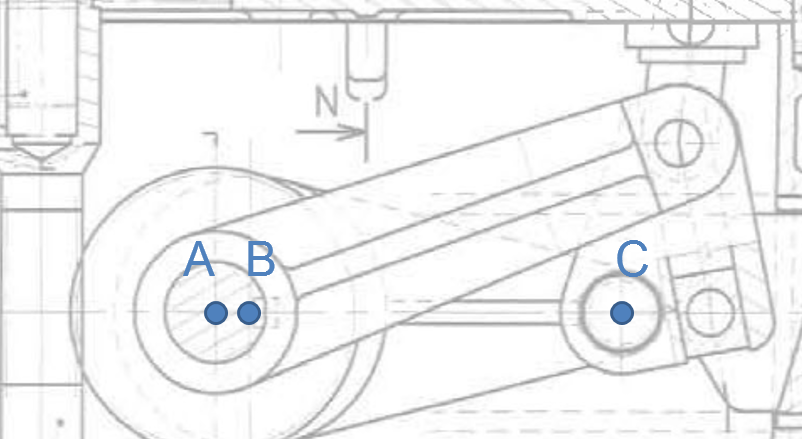
\includegraphics[width=0.8\linewidth]{img/pompe2}
\end{figure}


~\

\end{document}